
 \newpage
\subsection{SPI out}
This chapter will describe the SPI output module.

\subsubsection{Shift register}
The output consist of a 68 bit shift register where each cell in the register contains one D flip-flop and one multiplexer. As we have transistor schematics for both the flip flop and the multiplexer nothing had to be changed to the individual cells.

\begin{figure}[H]
\centering
\captionsetup{justification=centering}
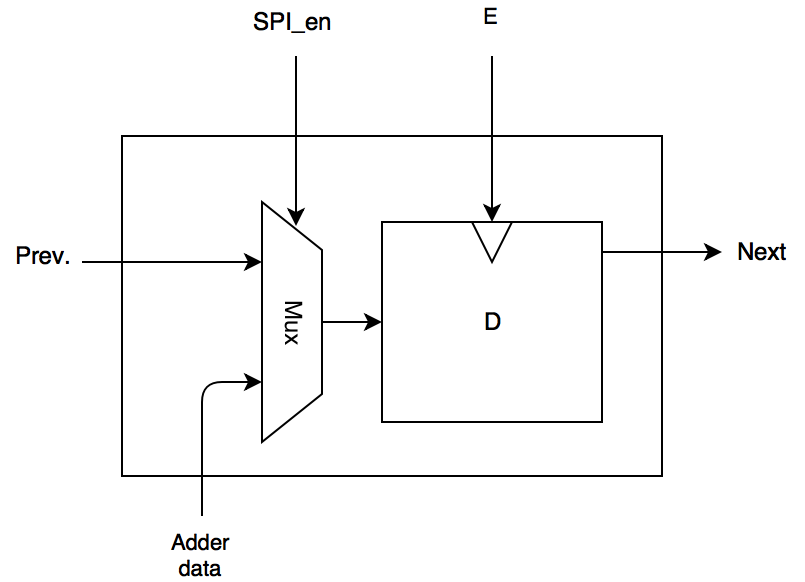
\includegraphics[scale=0.35]{../figures/MUX_DFF.png}
\caption{Shift register cell}
\label{mux_dff}
\end{figure}

\newpage

\subsubsection{Control logic}
As all verilogA code were replaced by transistor schematics, the problem with this design got exposed. Each of the four enable signal has a large fan out as they are connected to 17 cells in the shift register. \\
The solution was to size the the multiplexer generating the control signals. The last internal block that includes this multiplexer can be seen in Fig. \ref{and_mux}. 

\begin{figure}[H]
\centering
\captionsetup{justification=centering}
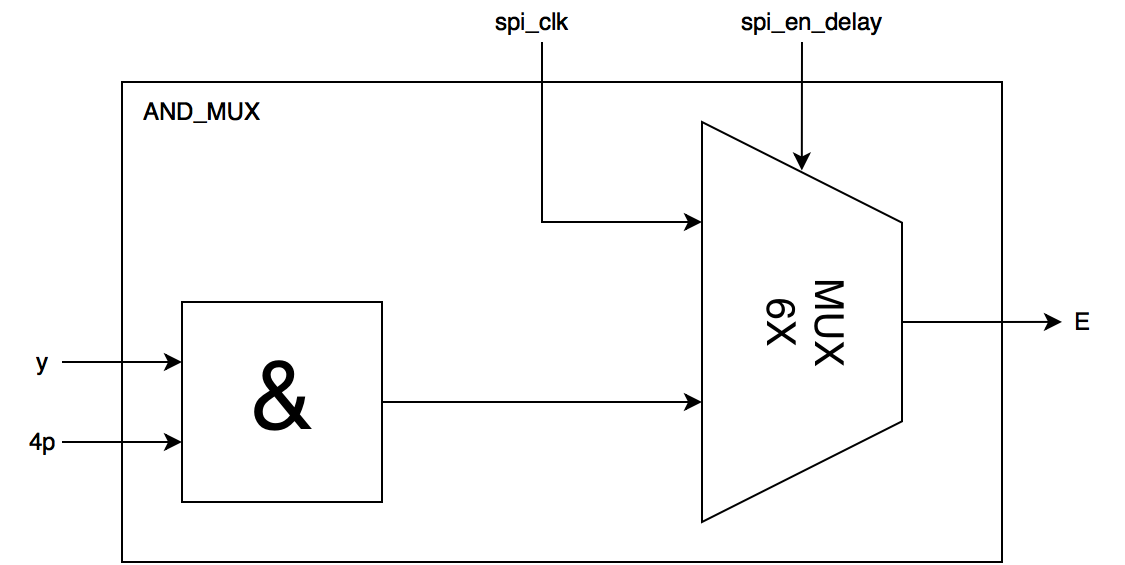
\includegraphics[scale=0.2]{../figures/AND_MUX.png}
\caption{Functional block containing an AND and a MUX.}
\label{and_mux}
\end{figure}

\raggedright By testing we found that a MUX that is approximately six times larger should be sufficient. In Fig. \ref{mux6x} the schematic of the sized multiplexer, implemented using NAND and an inverter is shown.

\begin{figure}[H]
\centering
\captionsetup{justification=centering}
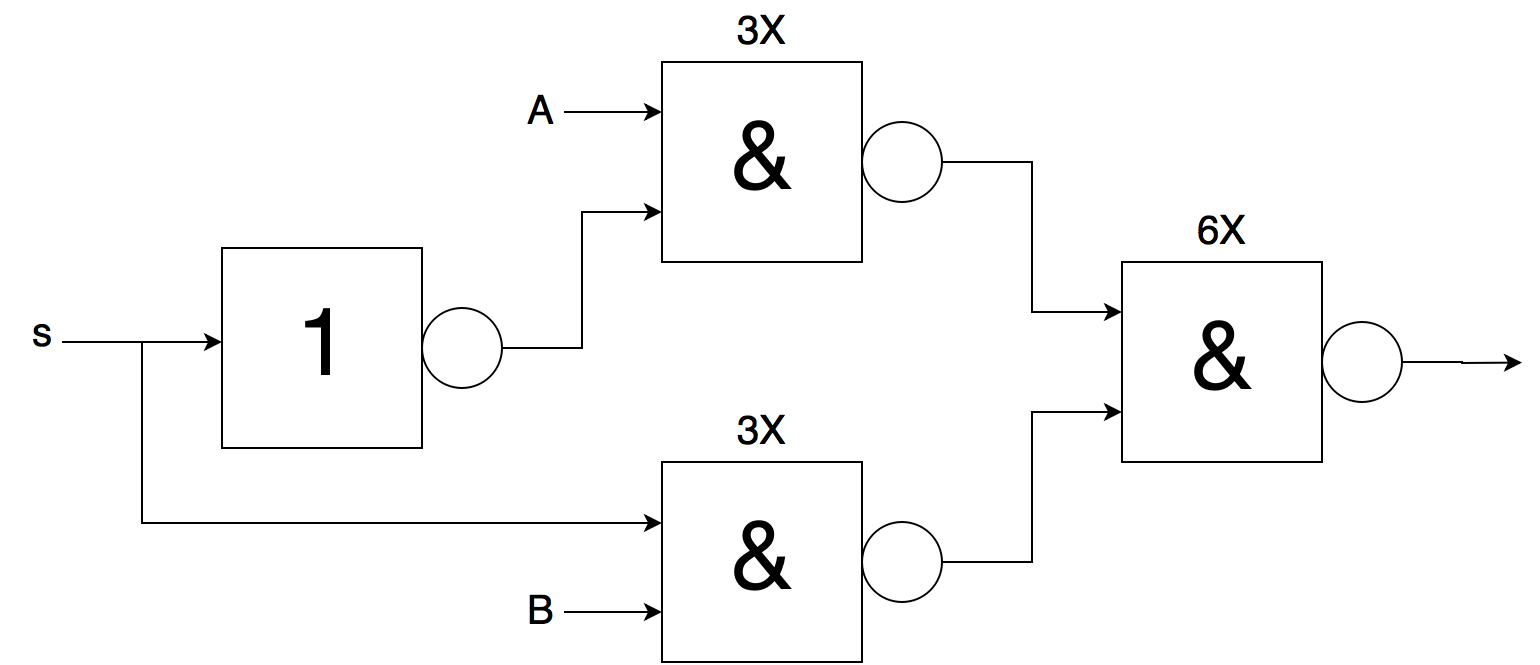
\includegraphics[scale=0.2]{../figures/MUX6X.png}
\caption{Sized multiplexer.}
\label{mux6x}
\end{figure}

\subsubsection{Protocol}
Due to a misunderstanding in the group regarding if the SPI clock should be kept high or low during the high time of the SPI enable signal, the data on the SPI output is now available for read already on the first falling edge of the SPI clock. This is possible because the the clock is kept low during high time of SPI enable so that the data can be written to the output at the first rising edge as usual but the first falling edge will come afterwards instead.



